\documentclass[11pt]{article}
\usepackage[margin=0.75in]{geometry}
\usepackage{amsmath}
\usepackage{enumitem}
\usepackage{color,soul}
\usepackage{multicol}
\usepackage{tikz}

\newcommand{\ds}{\displaystyle}

\begin{document}
\newcounter{enumCount}
\pagestyle{empty}
\subsection*{Math 141 - Homework 4 \hfill Name: \underline{\hspace*{2in}}}

\textit{Calculate the following limits exactly.}
\begin{multicols}{2}
\begin{enumerate}
\item $\ds \lim_{x \rightarrow 0} \frac{1}{2+\sin x}$
\item $\ds \lim_{x \rightarrow -1} \frac{2x-1}{x+2}$
\setcounter{enumCount}{\theenumi}
\end{enumerate}
\end{multicols}
\vfill

\noindent
\begin{multicols}{2}
\begin{enumerate}
\setcounter{enumi}{\theenumCount}
\item $\ds \lim_{x \rightarrow 2} \frac{x-2}{x^2-2x}$
\item $\ds \lim_{x \rightarrow 5} \frac{x^2 - 3x - 10}{x - 5}$
\setcounter{enumCount}{\theenumi}
\end{enumerate}
\end{multicols}
\vfill

\noindent
\begin{multicols}{2}
\begin{enumerate}
\setcounter{enumi}{\theenumCount}
\item $\ds \lim_{x \rightarrow 0} \frac{\sin x}{1+\cos x}$
\item $\ds \lim_{h \rightarrow 0} \frac{(1+h)^2 - 1}{h}$
\setcounter{enumCount}{\theenumi}
\end{enumerate}
\end{multicols}
\vfill

\begin{enumerate}
\setcounter{enumi}{\theenumCount}
\item Find $\ds \lim_{h \rightarrow 0} \frac{\frac{1}{a(a+h)} - \frac{1}{a^2}}{h}$ where $a$ is a non-zero constant.
\vfill


\item Determine the point(s), if any, at which each of the following functions is discontinuous. Classify any discontinuity as jump, removable, infinite, or other.
\begin{multicols}{3}
\begin{enumerate}
\item $\ds f(x) = \frac{x}{x^2 - x}$
\item $\ds g(x) = \cot 2x$
\item $\ds h(t) = t^{-1} + 1$
\end{enumerate}
\end{multicols}
\vfill

\newpage
\item Use the formula $\ds f'(a) = \lim_{x \rightarrow a} \frac{f(x)-f(a)}{x-a}$ to find the derivative of $f(x) = x^2$ at $a = 3$. 
\vfill
\vfill

\item Expand the polynomial $(x+h)^3$, i.e., multiply the factors $(x+h)(x+h)(x+h)$, then use your answer to find the derivative 
$$\dfrac{d}{dx} \, x^3 = \lim_{h \rightarrow 0} \frac{(x+h)^3 - x^3}{h}.$$
\vfill
\vfill


%\item Use the definition of derivative to find the derivative of the function $\ds f(x) = \frac{1}{x+1}$. 
%\vfill 

\item Use the graph below to find the following derivatives, or explain why they do not exist.

\begin{center}
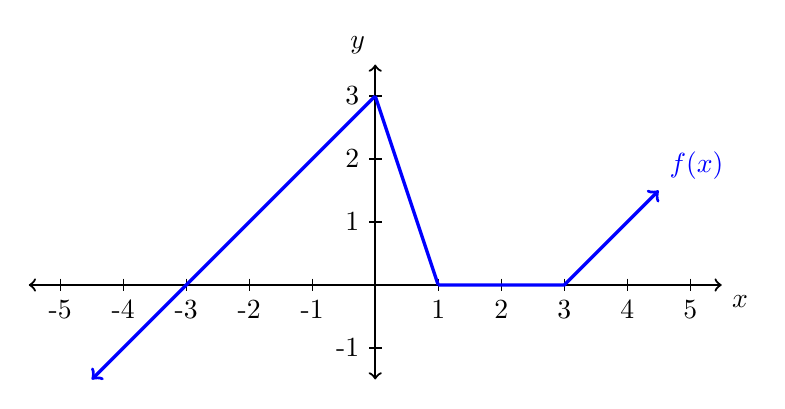
\begin{tikzpicture}[xscale=0.8,yscale=0.8]
\draw[thick,<->] (-5.5,0) -- (5.5,0) node[below right] {$x$};
\draw[thick,<->] (0,-1.5) -- (0,3.5) node[above left] {$y$};
\foreach \x in {1,2,3,4,5} {
  \draw (\x,0.1) -- (\x,-0.1) node[below] {\x};
}
\foreach \x in {-1,-2,-3,-4,-5} {
  \draw (\x,0.1) -- (\x,-0.1) node[below] {\x};
}
\foreach \y in {3,2,1,-1} {
  \draw (0.1,\y) -- (-0.1,\y) node[left] {\y};
}
\draw[very thick, blue, <-] (-4.5,-1.5) -- (0,3);
\draw[very thick, blue] (0,3) -- (1,0);
\draw[very thick, blue, ->] (1,0) -- (3,0) -- (4.5,1.5) node[above right] {$f(x)$};
\end{tikzpicture}
\end{center}
\begin{multicols}{5}
\begin{enumerate}
\item $f'(-1)$ 
\item $f'(0.5)$ 
\item $f'(1)$ 
\item $f'(2)$ 
\end{enumerate}
\end{multicols}
\bigskip

\item Sketch a rough graph of the derivative of the function shown in the graph below. Be sure to include numbers on the $x$ and $y$-axes.
\begin{flushleft}
\begin{tikzpicture}[xscale=0.8,yscale=0.8]
\draw[thick,<->] (-4.5,0) -- (4.5,0) node[below right] {$x$};
\draw[thick,<->] (0,-1.5) -- (0,3.5) node[above left] {$y$};
\foreach \x in {1,2,3,4} {
  \draw (\x,0.1) -- (\x,-0.1) node[below] {\x};
}
\foreach \x in {-1,-2,-3,-4,} {
  \draw (\x,0.1) -- (\x,-0.1) node[below] {\x};
}
\foreach \y in {3,2,1,-1} {
  \draw (0.1,\y) -- (-0.1,\y) node[left] {\y};
}
\draw[very thick,color=blue, <->] plot[domain=-4.2:4.2,samples=400] function {3/(1+x**2)};
\draw[blue] (2,2) node {$f(x)$};
\end{tikzpicture}
\end{flushleft}




\setcounter{enumCount}{\theenumi}
\end{enumerate}

\end{document}
